%%%%%%%%%%%%%%%%%%%%%%%%%%%%%%%%%%%%%%%%
% Class options                        %
%%%%%%%%%%%%%%%%%%%%%%%%%%%%%%%%%%%%%%%%
% Orientation:                         %
% portrait (default), landscape        %
%                                      %
% Paper size:                          %
% a0paper (default), a1paper, a2paper, %
% a3paper, a4paper, a5paper, a6paper   %
%                                      %
% Language:                            %
% english (default), norsk             %
%%%%%%%%%%%%%%%%%%%%%%%%%%%%%%%%%%%%%%%%
\documentclass[landscape]{uioposter}


\usepackage{lipsum}              % Dummy text
\usepackage{graphicx}
\usepackage{listings}
\usepackage{color}
\usepackage[figwidth=1.0\linewidth]{todonotes}  % Dummy image (and more!)
\usepackage[absolute, overlay]{textpos}            % Figure placement
\setlength{\TPHorizModule}{\paperwidth}
\setlength{\TPVertModule}{\paperheight}



\title{An Interactive Web-based GIS System to Evaluate Hurricane Inundation Impacts}
\author
{%
    Michael Bednarek \inst{1}
    \and
    Omid Alemi \inst{2}
    \and
    Saeed Moghimi \inst{3}
}
%% Optional:
\institute
{
    \inst{1}  Morristown Beard School (High school), 70 Whippany Rd, Morristown,
    NJ.\\
    \and
    \inst{2} School of Interactive Arts and Technology, Simon Fraser University,
    BC, Canada.\\
    \and
    \inst{3} NOAA National Ocean Service, Coast Survey Development Laboratory,
    Silver Spring, MD.\\
    
}
%% Or:
%\institute{Contact information}


%% Remove footline:
%\setbeamertemplate{footline}{}


\begin{document}
\begin{frame}
\begin{columns}[onlytextwidth]



%%% Col1

\begin{column}{\textwidth/3 - 2cm}
    
    \begin{block}{Introduction}
      The use of web-based geographic information systems (GIS) in a coastal
      environment can be beneficial for both coastal and scientific communities.
      With the collection of data from numerous sources and social media (e.g.
      FEMA API’s) and with access to model produced results for coastal
      inundation, we can generalize and interact with models to evaluate the
      impact of coastal events in an interactive and visual manner.
    \end{block}


    \begin{block}{System design}
     Bellow the diagram of the complete system from data collection to
     interaction with the user is given.
    
      \begin{figure}
         \centering
         %\hspace*{-20mm}
         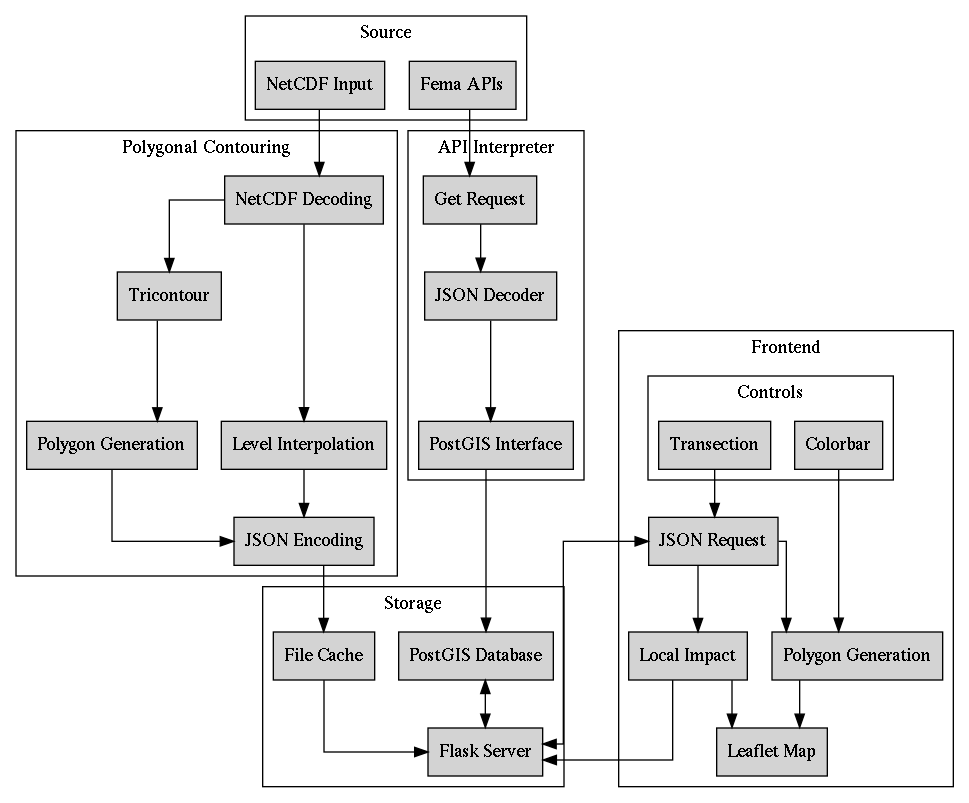
\includegraphics[scale=.9]{flowchart.png}
         \caption{Flowchart of the system.}   
         %\label{fig:timeseries_validation}
      \end{figure}
    
    
    \end{block}
    
        
\end{column}



%%% Col2

\begin{column}{\textwidth/3 - 2cm}
    
    \begin{block}{Data collection}
      Data from numerous sources including databases from The Federal
      Emergency Management Agency (FEMA), social media sources such
      as Instagram, and first hand collected model produced data from the
      NOAA's storm surge model results (ESTOFS), are collected to
      be used in later stages in the system.
    \end{block}
    
    
    \begin{block}{Model data processing}
      \begin{itemize}
        \item A collection of nodal values for maximum water surface elevation read from
      model generated NetCDF file.
      \item For both space saving and ease of manipulation, these values are
      grouped and vectorized to a collection of polygons.
      \item The polygons were organized for a given water surface levels.
      \item These polygons are then encoded into a
      JSON file including some general information about it’s size, value, and
      resolution.
      \end{itemize}
        
        
      \begin{figure}
         \centering
         %\hspace*{-20mm}
         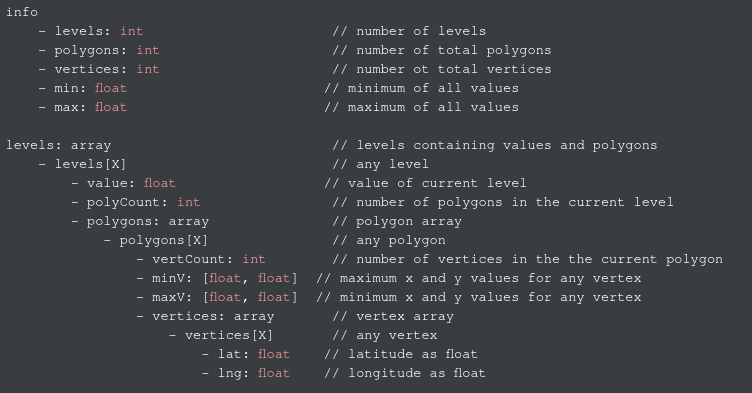
\includegraphics[scale=1.1]{screenshot1.png}
         \caption{Water surface levels polygons and their associate
      variables.}   
         %\label{fig:timeseries_validation}
      \end{figure}



    \end{block}

\end{column}


%%% Col2

\begin{column}{\textwidth/3 - 2cm}
    \begin{block}{Backend}
     \begin{itemize}
        \item A PostGIS server accomodates all the data generated
        from model results and observations collected from data sources.

        \item  A Flask web server is used to serve the compressed
        information created from the data processing phase. The server provides interface to number 
        of methods for interacting with the collected data. 
        
        \item The Shaply Python package is utilized to provide general
        definitions of polygons and other geometrical objects for interacting
        and generating transects and defining an area of interest to analys 
        land-use in comparison with maximum surge information.

     \end{itemize}
        
    \end{block}
    
     \begin{block}{Frontend}
        The graphical interface is written in pure HTML / JavaScript using
        Leaflet package to provide an intuitive way of interacting with the
        data. It allows the user to foremost graph inundation and flood
        levels, as well as transect values, select regions, and compare with 
        land use information. 
    \end{block}
    

    \begin{block}{Outlook}
    We are planning to further develop:
    \begin{itemize}
  \item A more advanced polygonal area selection
  \item A flexible colorbar UI elements
  \item A direct NetCDF caching
  \item Implement a seamless connection to data APIs (e.g. FEMA, NOAA) 
\end{itemize}
    
    \end{block}
\end{column}


\end{columns}


\begin{textblock}{0.5}(0.025, 0.9575)
    \color{white}
    \sffamily
    \textbf{Github Organization}
    \\
    https://github.com/earth-sys-ai
\end{textblock}


\end{frame}
\end{document}